%%%%%%%%%%%%%%%%%%%%%%%%%%%%%%%%%%%%%%%%%
% Dreuw & Deselaer's Poster
% LaTeX Template
% Version 1.0 (11/04/13)
%
% Created by:
% Philippe Dreuw and Thomas Deselaers
% http://www-i6.informatik.rwth-aachen.de/~dreuw/latexbeamerposter.php
%
% This template has been downloaded from:
% http://www.LaTeXTemplates.com
%
% License:
% CC BY-NC-SA 3.0 (http://creativecommons.org/licenses/by-nc-sa/3.0/)
%
%%%%%%%%%%%%%%%%%%%%%%%%%%%%%%%%%%%%%%%%%

%----------------------------------------------------------------------------------------
%	PACKAGES AND OTHER DOCUMENT CONFIGURATIONS
%----------------------------------------------------------------------------------------

\documentclass[final,hyperref={pdfpagelabels=false}]{beamer}

\usepackage[orientation=landscape,size=a0,scale=1.4]{beamerposter} % Use the beamerposter package for laying out the poster with a portrait orientation and an a0 paper size

\usetheme{I6pd2} % Use the I6pd2 theme supplied with this template

\usepackage[english]{babel} % English language/hyphenation

\usepackage{amsmath,amsthm,amssymb,latexsym} % For including math equations, theorems, symbols, etc

%\usepackage{times}\usefonttheme{professionalfonts}  % Uncomment to use Times as the main font
%\usefonttheme[onlymath]{serif} % Uncomment to use a Serif font within math environments

\boldmath % Use bold for everything within the math environment

\usepackage{booktabs} % Top and bottom rules for tables

\graphicspath{{figures/}} % Location of the graphics files

\usecaptiontemplate{\small\structure{\insertcaptionname~\insertcaptionnumber: }\insertcaption} % A fix for figure numbering


% Additional packages
\usepackage[misc]{ifsym}

% commands
\newcommand{\todo}[1]{\textcolor{red}{\{\textbf{#1}\}}}

%----------------------------------------------------------------------------------------
%	TITLE SECTION 
%----------------------------------------------------------------------------------------

\title{\huge The Intrinsic Manifolds of Radiological Images and their Role in Deep Learning} % Poster title

\author{Nicholas Konz\textsuperscript{1*(\Letter)}\and Hanxue Gu\textsuperscript{1} \and Haoyu Dong\textsuperscript{2} \and Maciej Mazurowski\textsuperscript{1,2,3,4(\Letter)} } % Author(s)

\institute{\textsuperscript{1}Department of Electrical and Computer Engineering, \textsuperscript{2}Department of Radiology, \textsuperscript{3}Department of Computer Science, \textsuperscript{4}Department of Biostatistics \& Bioinformatics,\\Duke University, North Carolina, USA} % Institution(s)

%----------------------------------------------------------------------------------------
%	FOOTER TEXT
%----------------------------------------------------------------------------------------

\newcommand{\leftfoot}{http://www.LaTeXTemplates.com} % Left footer text

\newcommand{\rightfoot}{} % Right footer text

%----------------------------------------------------------------------------------------

\begin{document}

\addtobeamertemplate{block end}{}{\vspace*{2ex}} % White space under blocks

\begin{frame}[t] % The whole poster is enclosed in one beamer frame

\begin{columns}[t] % The whole poster consists of two major columns, each of which can be subdivided further with another \begin{columns} block - the [t] argument aligns each column's content to the top

\begin{column}{.02\textwidth}\end{column} % Empty spacer column

\begin{column}{.3\textwidth} % The first column

\begin{block}{Introduction}

\begin{itemize}
\item \textbf{The Manifold Hypothesis}
\end{itemize}

\end{block}

\begin{block}{Objectives}

\begin{enumerate}
\item 
\end{enumerate}

\end{block}

\begin{block}{Datasets and Tasks}

\begin{figure}
    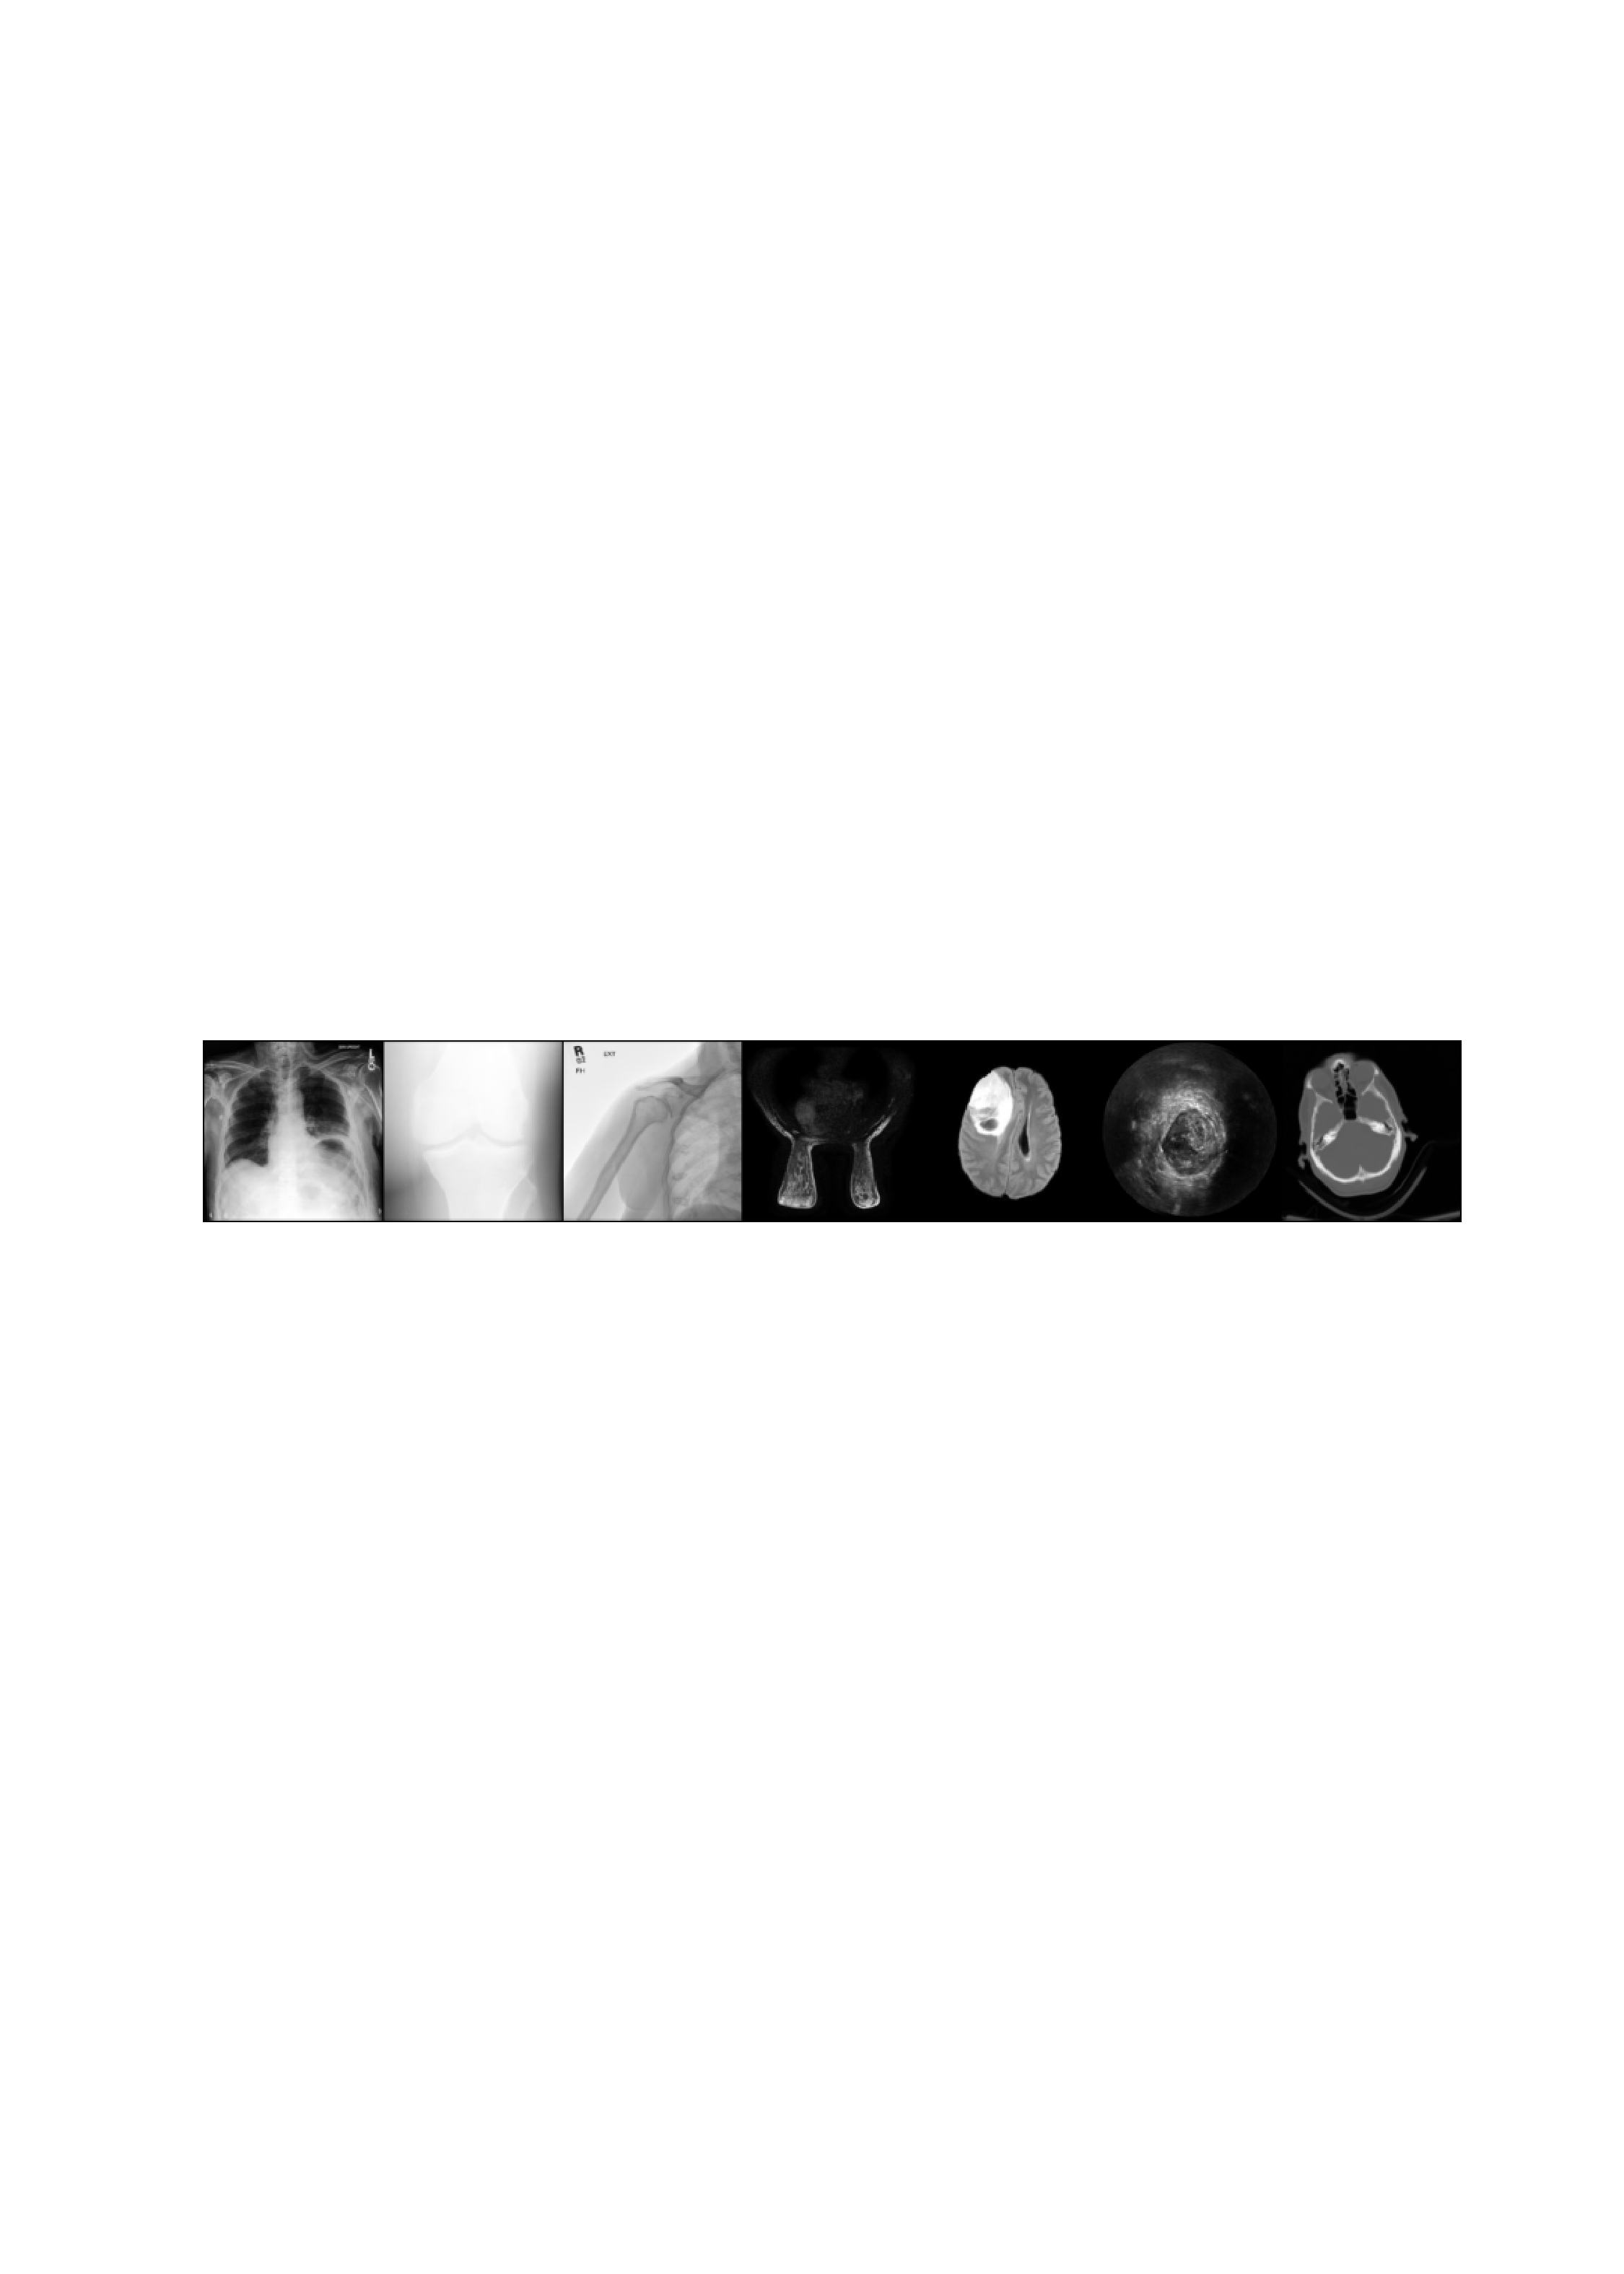
\includegraphics[width=0.95\linewidth]{frompaper/data_eg_1row.pdf}
     \caption{Samples from our evaluated datasets.}
\end{figure}

\begin{columns} % Subdivide the first main column
\begin{column}{.54\textwidth} % The first subdivided column within the first main column
\begin{itemize}
\item Vestibulum nisl, quis euismod velit eros in ligula.
\begin{itemize}
\item Cras rhoncus quam et augue convallis in elementum urna tincidunt.
\end{itemize}
\item Proin ut vestibulum augue.
\begin{itemize}
\item Donec dapibus sagittis neque eu ultrices.
\end{itemize}
\end{itemize}
\end{column}

\begin{column}{.43\textwidth} % The second subdivided column within the first main column
\centering
\begin{figure}

\includegraphics[width=0.8\linewidth]{placeholder.jpg}
\caption{Figure caption}
\end{figure}
\end{column}
\end{columns} % End of the subdivision

\begin{itemize}
\item Curabitur sapien ligula, faucibus in feugiat quis, vestibulum a turpis.
\begin{itemize}
\item Phasellus quis nunc neque. Suspendisse mauris diam, suscipit non gravida in, placerat id enim. Ut nec ipsum in lectus ultrices sagittis.
\item Ut nec ipsum in lectus ultrices sagittis.
\item Phasellus quis nunc neque.
\end{itemize}
\end{itemize}

\end{block}

\begin{block}{}

\end{block}

\begin{block}{Estimating Intrinsic Dimension}

\begin{itemize}
\item Maecenas Ultricies Feugiat Velit Non Mattis.
\begin{itemize}
\item Duis
\begin{align*}
X \rightarrow r(X) & = \arg \max_{c} \Big\{ \max_n \big\{ \sum_{x_i \in X} \delta(x_i,Y_{n,c})\big\} \Big\} 
\end{align*}
\item Cras
\end{itemize}
\item Fusce
\end{itemize}

\end{block}

%----------------------------------------------------------------------------------------

\end{column} % End of the first column

\begin{column}{.03\textwidth}\end{column} % Empty spacer column
 
\begin{column}{.3\textwidth} % The second column

\begin{figure}
    
\includegraphics[width=0.95\linewidth]{placeholder.jpg}
     \caption{\todo{some visualization of intrinsic manifold dimension}}
\end{figure}

\begin{block}{Result 1: Radiological vs. Natural Image Intrinsic Dimension}
\begin{figure}
    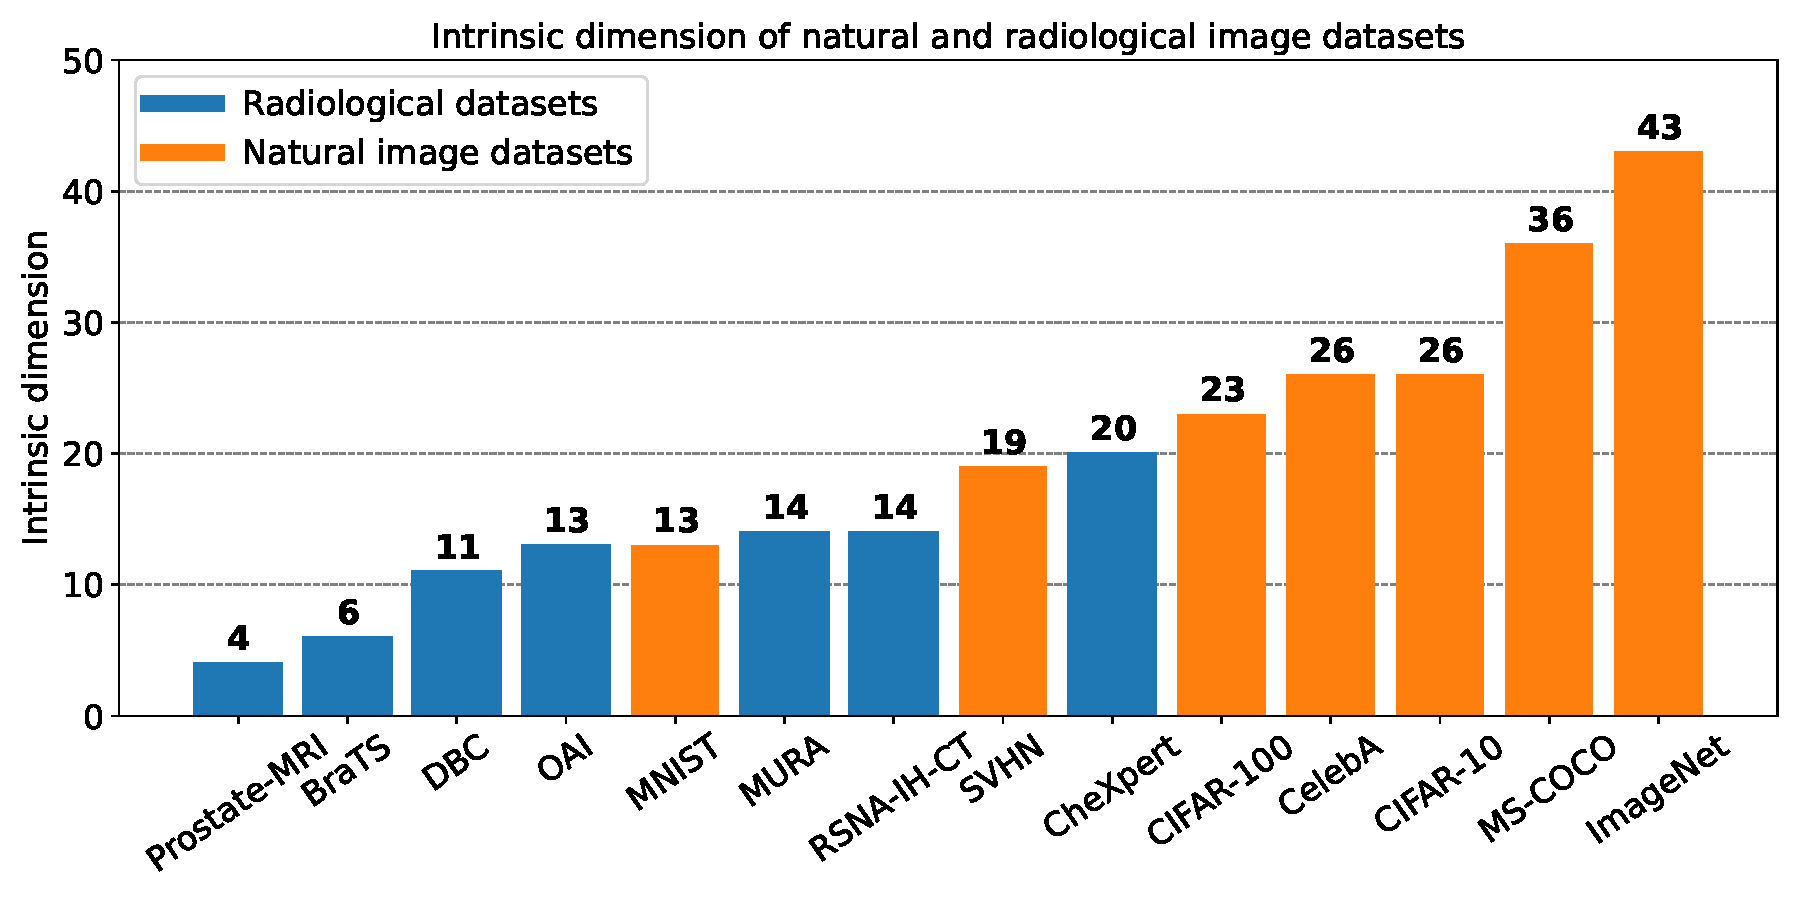
\includegraphics[width=0.95\linewidth]{frompaper/ID.pdf}
     \caption{Intrinsic dimension of \textcolor{paperblue}{radiological} and \textcolor{paperorange}{natural} \cite{pope2021intrinsic} image datasets.}
\end{figure}

\end{block}

%----------------------------------------------------------------------------------------

\end{column} % End of the second column

\begin{column}{.03\textwidth}\end{column} % Empty spacer column
 
\begin{column}{.3\textwidth} % The third column


\begin{block}{Result 2: Radiological vs. Natural Image Intrinsic Dimension}

\begin{figure}
    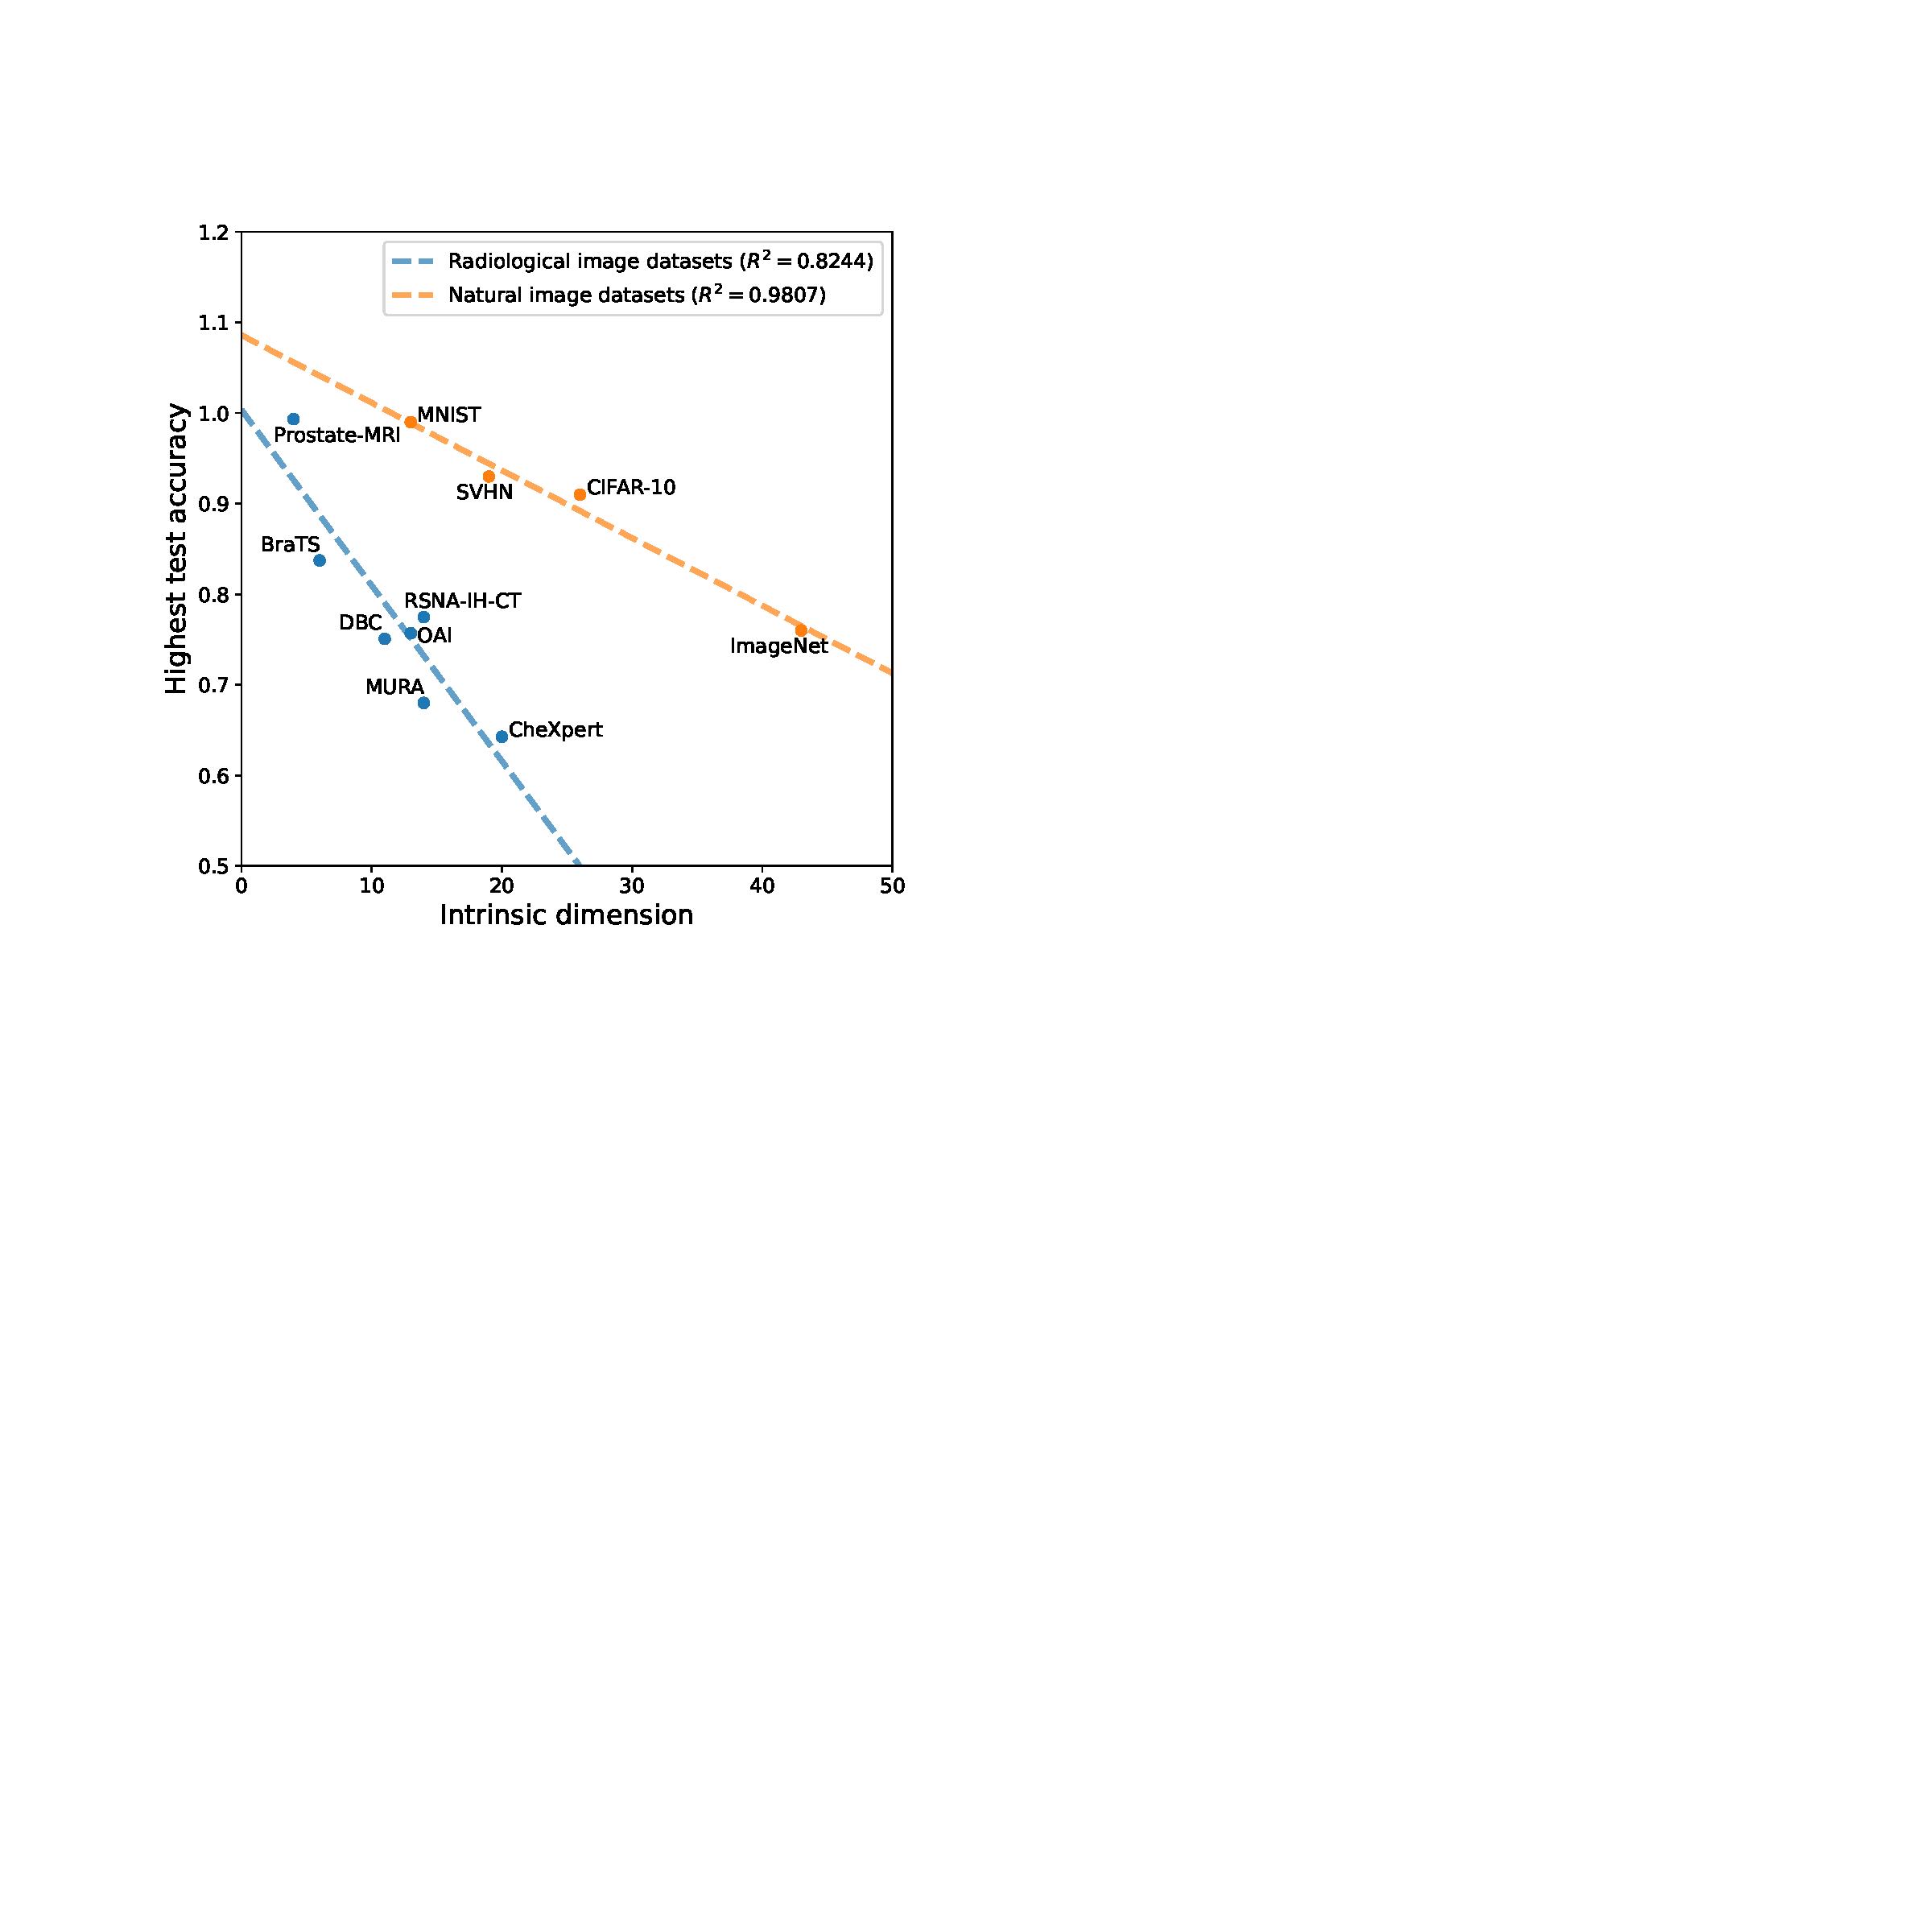
\includegraphics[width=0.95\linewidth]{frompaper/main_fig_multi_0.pdf}
     \caption{Linearity of model generalization ability with respect to dataset intrinsic dimension, for \textcolor{paperblue}{radiological} and \textcolor{paperorange}{natural} image datasets ($N_\text{train}=2000$ on ResNet-18).}
\end{figure}

\todo{numerical evidence showing how these relationships didn't change with model, dataset size, task, etc (see paper)}

\end{block}

\begin{block}{Open Questions}

\begin{itemize}
\item Opet volutpat ligula.
\end{itemize}

\end{block}


\begin{block}{References}
        
% \nocite{*} % Insert publications even if they are not cited in the poster
\small{\bibliographystyle{unsrt}
\bibliography{mainbib}}

\end{block}

\setbeamercolor{block title}{fg=black,bg=orange!70} % Change the block title color

\begin{block}{Contact Information}

\begin{itemize}
\item Web: \todo{lab website}
\item Email: \href{mailto:nicholas.konz@duke.edu}{nicholas.konz@duke.edu}
\end{itemize}

\end{block}
\end{column} % End of the third column


\begin{column}{.015\textwidth}\end{column} % Empty spacer column

\end{columns} % End of all the columns in the poster

\end{frame} % End of the enclosing frame

\end{document}